
\section{Recursive neural network models} \label{methods}

We study neural models that adhere to the linguistic \ii{principle of
 compositionality}, which says that the meanings for complex
expressions are derived from the meanings of their constituent parts
via specific composition functions \cite{Partee84,Janssen97}. In our
distributed setting, word meanings are vectors of length $n$. The
composition function maps pairs of them to single vectors of length $n$, 
which can then be merged again to represent more complex
phrases. Once the entire sentence-level representation has been
derived, it serves as a fixed-length input for some subsequent function.

We use the model architecture depicted in Figure~\ref{sample-figure}. 
The two phrases being compared are processed separately using a pair 
of recursive networks that share a single set of parameters. 
The resulting vectors are fed into a separate comparison
layer (fixed at 75 dimensions) that is meant to generate a feature vector capturing the
relation between the two phrases. The output of this layer is then
given to a softmax classifier, which in turn produces a hypothesized
distribution over the seven relations represented in Table~\ref{b-table}.

For a composition layer, we evaluate models with both the plain neural
network layer function \eqref{rnn} and a more powerful extension, the RNTN layer function
\eqref{rntn} proposed in \newcite{chen2013learning}. A $\tanh$ nonlinearity is applied to the output of the layer function.
%
\begin{gather} \label{rnn}
\vec{y}_{\textit{RNN}} = f(\mathbf{M} [\vec{x}^{(l)}; \vec{x}^{(r)}] + \vec{b}) \\
\label{rntn}
\vec{y}_{\textit{RNTN}} = \vec{y}_{\textit{RNN}} + f(\vec{x}^{(l)T} \mathbf{T}^{[1 \ldots n]} \vec{x}^{(r)})
\end{gather} 
%
Here, $\vec{x}^{(l)}$ and $\vec{x}^{(r)}$ are the column vector
representations for the left and right children of the node, and
$\vec{y}$ is the node's output.  The RNN concatenates them, multiplies
them by an $n \times 2n$ matrix of learned weights, adds a bias $\vec{b}$, and applies the
element-wise non-linearity to the resulting vector. The RNTN adds a learned third-order tensor 
$\mathbf{T}$, dimension $n \times n \times n$, modeling
multiplicative interactions between the child vectors.

The comparison layer uses the same layer function as the
composition layers (either an NN layer or an NTN layer) with
independently learned parameters and a separate nonlinearity function.
Rather than use a $\tanh$ nonlinearity here, we use a rectified linear function. In
particular, we use the leaky rectified linear function
\shortcite{maasrectifier}: $f(\vec{x})=\max(\vec{x}, 0) +
0.01\min(\vec{x}, 0)$, applied element-wise.

To run the model forward and label a pair of phrases, the structure of
the lower layers of the network is assembled so as to mirror the tree
structures provided for each phrase. The word vectors are then looked
up from the vocabulary matrix $V$ (one of the model parameters), and
the composition and comparison functions are used to pass information
up the tree and into the classifier at the top. For an objective
function, we use the negative log of the probability assigned to the
correct label.

% Removed 'minibatch' -> For two of the experiments, we use minibatches
% of size 1, which doesn't really count.
We train the model using stochastic gradient descent (SGD)
with learning rates computed using ADADELTA \cite{zeiler2012adadelta}.
The parameters (including the vocabulary) are initialized randomly.
Because the classes are not balanced in general, we report performance
using both accuracy and macroaveraged F1, since the latter emphasizes
 performance on infrequent classes. We compute macroaveraged F1 
as the harmonic mean of mean precision and mean recall, both computed
for all classes for which there is test data, setting precision to 0 
where it is not defined. Source code and generated data will be released
after the review period.

\begin{figure*}[tp]
  \centering
 % 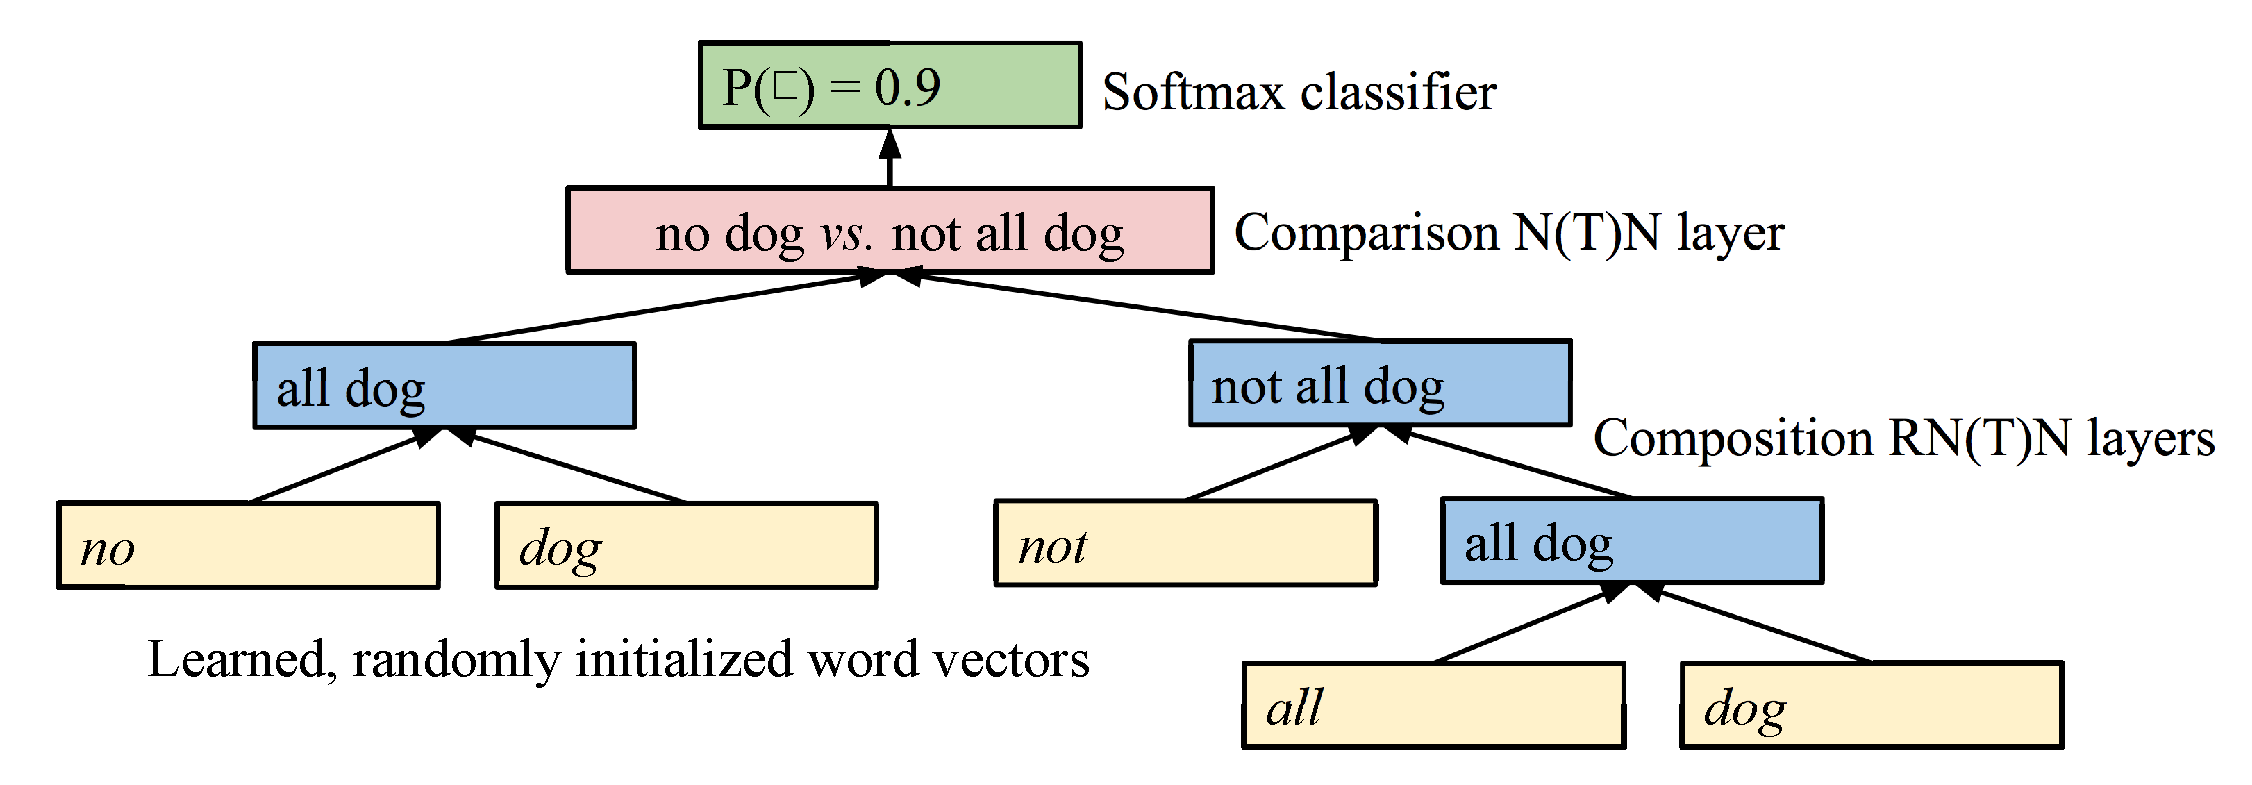
\includegraphics[scale=0.35]{model.eps}
  \footnotesize

\newcommand{\labeledtreenode}[4][3.5]{\put(#2){\makebox(0,0){{\fcolorbox{black}{#4}{\makebox(#1,0.3){#3}}}}}}

\newcommand{\textlabel}[4][3.5]{\put(#2){\makebox(0,0){{\fcolorbox{white}{white}{\makebox(#1,0.3){#3}}}}}}

\definecolor{lexcolor}{HTML}{F5F7C4}
\definecolor{compositioncolor}{HTML}{BBEBFF}
\definecolor{comparisoncolor}{HTML}{FFC895}
\definecolor{softmaxcolor}{HTML}{A5FF8A}


\setlength{\unitlength}{0.61cm}
\begin{picture}(21,7.5)
  
  \labeledtreenode[2.4]{11.5,7}{$P(\sqsubset) = 0.8$}{softmaxcolor}  
  \put(11.5,5.7){\vector(0,1){1}}  
  \labeledtreenode[7.85]{11.5,5.4}{all reptiles walk \emph{vs.}~some turtles move}{comparisoncolor}


  \textlabel{8,7}{Softmax classifier}{black}
  \textlabel{4.5,5.4}{Comparison N(T)N layer}{black}
      
  \textlabel{11.75,3.6}{Composition RN(T)N layers}{black}

  \textlabel{5,0.1}{Learned, randomly initialized word vectors}{black}
  
  %%%%%%%%%%%%%%%%%%%%%%%%%%%%%%%%%%%%%%%%%%%%%%%%%%
    
  \put(1.75,1.35){\vector(2,1){1.7}}
  \labeledtreenode{1.75,1}{all}{lexcolor}

  \put(6,1.35){\vector(-2,1){1.7}}
  \labeledtreenode{6,1}{reptiles}{lexcolor}

  \put(4,2.75){\vector(2,1){1.7}}
  \labeledtreenode{4,2.5}{all reptiles}{compositioncolor}

  \put(8.25,2.75){\vector(-2,1){1.7}}
  \labeledtreenode{8.25,2.5}{walk}{lexcolor}

  \put(6.25,4.25){\vector(4,1){3.25}}
  \labeledtreenode{6.25,3.9}{all reptiles walk}{compositioncolor}
  
  %%%%%%%%%%%%%%%%%%%%%%%%%%%%%%%%%%%%%%%%%%%%%%%%%%%

  \put(12.75,1.35){\vector(2,1){1.7}}
  \labeledtreenode{12.75,1}{some}{lexcolor}

  \put(17,1.35){\vector(-2,1){1.7}}
  \labeledtreenode{17,1}{turtles}{lexcolor}

  \put(15,2.75){\vector(2,1){1.7}}
  \labeledtreenode{15,2.5}{some turtles}{compositioncolor}

  \put(19.25,2.75){\vector(-2,1){1.7}}
  \labeledtreenode{19.25,2.5}{move}{lexcolor}
          
  \put(17.25,4.25){\vector(-4,1){3.25}}
  \labeledtreenode{17.25,3.9}{some turtles move}{compositioncolor}
  
\end{picture}



  \caption{The model structure used to compare \ii{((all reptiles) walk)} and \ii{((some turtles) move)}. 
    The same structure is used for both the RNN and RNTN layer functions.} 
  \label{sample-figure}
\end{figure*}
